\chapter{La biodiversidad a todas las escalas}\label{ch:g10:biodiversity-scales}

Coloca un cuadrado de cuerda de un metro de lado sobre un césped y
cuenta lo que crece dentro: hierba, claro, pero también trébol,
margaritas, un diente de león, llantén, musgo y, si miras con una lupa,
una docena de insectos y un caracol. Pasa el cuadrado al asfalto del
aparcamiento: nada, o una mala hierba en una grieta. Pásalo a un prado
viejo que nunca se ha arado: cuarenta \omterm{def:g10:biodiversity-scales:species}{especies} de plantas, y los
insectos incontables. La palabra que designa lo que mide el cuadrado es
\emph{\omterm{def:g10:biodiversity-scales:biodiversity}{biodiversidad}}, y este capítulo trata de cómo se mide, a qué
escalas existe y por qué no es ni fija ni está garantizada.

\section{Tres escalas de diversidad}

\begin{definition}[Biodiversidad]\label{def:g10:biodiversity-scales:biodiversity}
La \emph{biodiversidad}\index{biodiversidad} es la diversidad de los
seres vivos, considerada a tres escalas:
\begin{itemize}
  \item la diversidad de \emph{ecosistemas}\index{ecosistema} --- de
        las comunidades vivas y de los medios que ocupan (una charca,
        un hayedo, un arrecife de coral, un prado), cada uno con su
        propio conjunto de \omterm{def:g10:biodiversity-scales:species}{especies};
  \item la diversidad de \omterm{def:g10:biodiversity-scales:species}{especies} dentro de un
        ecosistema o en la Tierra --- el número de \omterm{def:g10:biodiversity-scales:species}{especies} y su
        abundancia relativa;
  \item la \emph{diversidad genética}\index{diversidad genética}
        dentro de una \omterm{def:g10:biodiversity-scales:species}{especie} --- el número de \omterm{def:g10:universal-dna:gene}{alelos} de sus \omterm{def:g10:universal-dna:gene}{genes} y la
        manera en que se reparten entre sus individuos y sus
        poblaciones.
\end{itemize}
\end{definition}

\begin{omfigure}
\begin{tikzpicture}[font=\small, >=Stealth]
  \node[draw, rounded corners, thick, fill=omMeth!8, minimum width=11.4cm, minimum height=4.9cm] (eco) at (0,0) {};
  \node[anchor=north west, font=\small\bfseries] at (eco.north west) {\ ecosistemas: charca, bosque, arrecife, prado\dots};
  \node[draw, rounded corners, thick, fill=omDef!10, minimum width=8.2cm, minimum height=3.2cm] (sp) at (0.6,-0.45) {};
  \node[anchor=north west, font=\small\bfseries] at (sp.north west) {\ especies de un ecosistema};
  \foreach \x/\t in {-2.6/rana, -1.1/tritón, 0.4/libélula, 1.9/carrizo, 3.4/nenúfar}
    \node[draw, fill=white, rounded corners=2pt, font=\scriptsize] at (\x,-0.3) {\t};
  \node[draw, rounded corners, thick, fill=omProp!12, minimum width=6.4cm, minimum height=1.2cm] (al) at (1.0,-1.35) {};
  \node[anchor=west, font=\scriptsize\bfseries] at (al.west) {\ alelos de una especie:};
  \foreach \x/\t in {1.6/a, 2.2/b, 2.8/c, 3.4/d, 4.0/e}
    \node[draw, circle, fill=white, inner sep=1.5pt, font=\scriptsize] at (\x,-1.35) {\t};
\end{tikzpicture}

{\small Las tres escalas encajadas de la \omterm{def:g10:biodiversity-scales:biodiversity}{biodiversidad}. Perder una
charca es perder una comunidad de \omterm{def:g10:biodiversity-scales:species}{especies}; perder una \omterm{def:g10:biodiversity-scales:species}{especie} es
perder todos sus \omterm{def:g10:universal-dna:gene}{alelos}; perder \omterm{def:g10:universal-dna:gene}{alelos} empobrece a una \omterm{def:g10:biodiversity-scales:species}{especie} que
sigue existiendo.}
\end{omfigure}

\begin{definition}[Especie]\label{def:g10:biodiversity-scales:species}
Una \emph{especie}\index{especie} es un grupo de seres vivos que se parecen entre sí,
pueden reproducirse juntos y dan descendencia fértil; dos poblaciones
que no pueden cruzarse, o cuyos híbridos son estériles, son especies
distintas. En la práctica --- con los fósiles, con las bacterias, con
organismos a los que nunca se ha visto reproducirse --- las especies se
reconocen por sus caracteres compartidos, y el
\cref{ch:g12:selection-drift-speciation} mostrará que el límite no
siempre es nítido.
\end{definition}

\begin{example}[Caballo, burro, mulo]\label{ex:g10:biodiversity-scales:mule}
Un caballo y un burro se parecen y pueden cruzarse: su descendiente es
el mulo. Pero el mulo es estéril, así que caballo y burro son dos
\omterm{def:g10:biodiversity-scales:species}{especies}. Un caniche y un lebrel irlandés no se parecen en nada, se
cruzan sin dificultad y dan cachorros fértiles: una sola \omterm{def:g10:biodiversity-scales:species}{especie}, el
perro --- que además puede cruzarse con el lobo, su antepasado.
\end{example}

\section{La diversidad de especies}

\begin{proposition}[Contar especies]\label{prop:g10:biodiversity-scales:count}
Se han descrito y nombrado unos dos millones de \omterm{def:g10:biodiversity-scales:species}{especies}. La mayoría
son insectos (más de un millón), seguidos de las plantas (unas
300\,000), los hongos, los arácnidos y los moluscos; los vertebrados,
el grupo que mejor conocemos, son unos 70\,000, de los que 6\,400 son
mamíferos. El número de \omterm{def:g10:biodiversity-scales:species}{especies} aún sin describir se estima, a partir
del ritmo al que se encuentran nuevas, en varios millones más --- quizá
de ocho a diez millones de \omterm{def:g10:biodiversity-scales:species}{especies} eucariotas en total, más una
diversidad inmensa y casi sin contar de bacterias.
\end{proposition}
\admitted

\begin{omfigure}
\begin{tikzpicture}
\begin{axis}[
  xbar, bar width=7pt,
  width=0.8\linewidth, height=6.4cm,
  axis x line=bottom, axis y line=left,
  xmin=0, xmax=1200,
  xlabel={especies descritas (en miles)},
  xlabel style={font=\small, at={(axis description cs:0.5,-0.1)}, anchor=north},
  symbolic y coords={mamíferos, aves, peces, moluscos, arácnidos, hongos, plantas, insectos},
  ytick=data, tick label style={font=\small},
  enlarge y limits=0.1,
  nodes near coords, nodes near coords style={font=\scriptsize, anchor=west},
  xtick={0,200,400,600,800,1000,1200},
]
\addplot[fill=omDef!55, draw=omDef] coordinates
  {(6.4,mamíferos) (11,aves) (34,peces) (85,moluscos) (100,arácnidos)
   (150,hongos) (300,plantas) (1000,insectos)};
\end{axis}
\end{tikzpicture}

{\small \omterm{def:g10:biodiversity-scales:species}{Especies} descritas en algunos grupos grandes, en miles. Los
grupos que mejor conocemos son los más pequeños; solo los insectos
superan a todos los vertebrados en proporción de quince a uno.}
\end{omfigure}

\begin{method}[Medir la diversidad de un lugar]\label{met:g10:biodiversity-scales:sampling}
Un lugar nunca se cuenta entero; se \emph{muestrea}.
\begin{enumerate}
  \item Elige una unidad de muestreo adaptada a los organismos: un
        cuadrado de \qty{1}{m^2} para las plantas de un prado, un
        barrido de manga para los insectos, un tamiz de tierra para las
        lombrices, un tramo de transecto para las aves.
  \item Coloca las unidades al azar o a intervalos regulares, y en
        número suficiente para que añadir una más cambie poco el total.
  \item En cada una, identifica y cuenta. Dos números describen la
        muestra: la \emph{riqueza de \omterm{def:g10:biodiversity-scales:species}{especies}}, el número de \omterm{def:g10:biodiversity-scales:species}{especies}
        encontradas, y la \emph{abundancia relativa} de cada una ---
        un lugar donde una \omterm{def:g10:biodiversity-scales:species}{especie} supone el 95\% de los individuos es
        menos diverso que otro donde diez \omterm{def:g10:biodiversity-scales:species}{especies} se los reparten por
        igual, aun con la misma riqueza.
  \item Compara lugares solo con el mismo método, el mismo esfuerzo y
        la misma estación.
\end{enumerate}
\end{method}

\begin{example}[Dos céspedes]\label{ex:g10:biodiversity-scales:lawns}
Diez cuadrados en el césped segado de un colegio: 6 \omterm{def:g10:biodiversity-scales:species}{especies} de
plantas, de las que la hierba cubre el 90\%. Diez cuadrados en un
ribazo sin segar contiguo: 23 \omterm{def:g10:biodiversity-scales:species}{especies}, ninguna por encima del 30\%. El
ribazo es más rico y más equilibrado; la diferencia no está en el suelo
ni en el clima, que son los mismos, sino en la siega, que elimina toda
planta incapaz de florecer a ras de suelo.
\end{example}

\begin{omfigure}
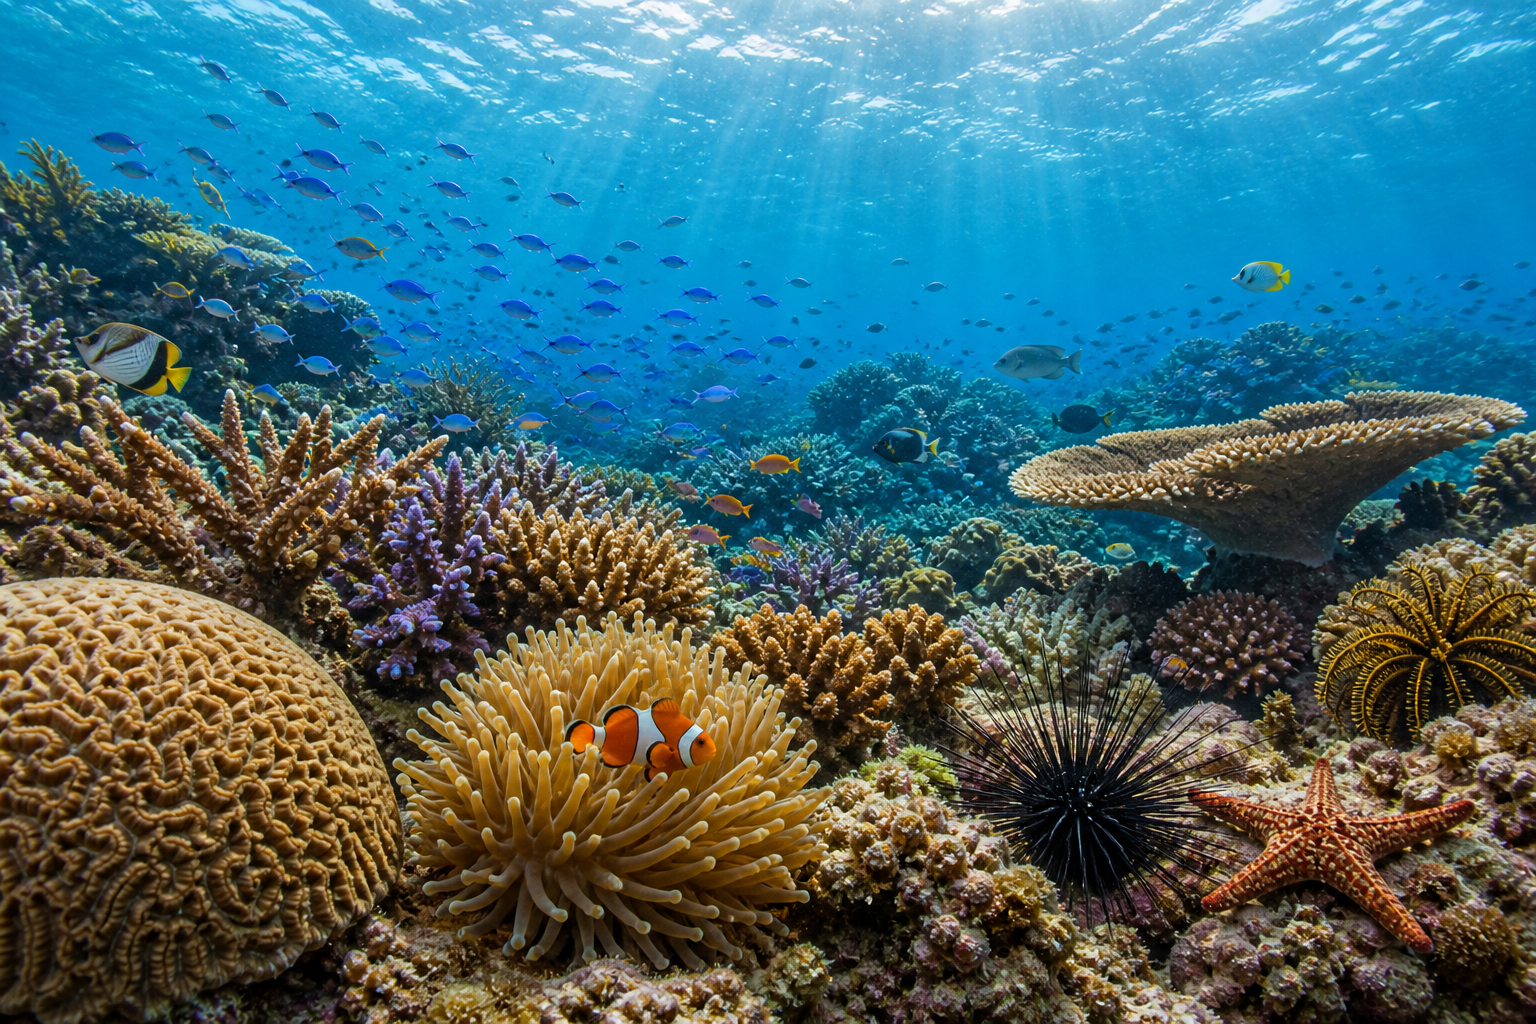
\includegraphics[width=0.66\linewidth]{images/book2/ai/g10-biodiv-coral-reef.png}

{\small Un arrecife de coral: en unos pocos metros cuadrados, corales,
peces, moluscos, equinodermos y anémonas de decenas de \omterm{def:g10:biodiversity-scales:species}{especies}. Los
arrecifes albergan un cuarto de todas las \omterm{def:g10:biodiversity-scales:species}{especies} marinas en una
milésima parte del fondo oceánico.}
\end{omfigure}

\section{La diversidad genética dentro de una especie}

\begin{proposition}[Los individuos de una especie no son idénticos]\label{prop:g10:biodiversity-scales:genetic}
Dentro de una \omterm{def:g10:biodiversity-scales:species}{especie}, la mayoría de los \omterm{def:g10:universal-dna:gene}{genes} existen en varios \omterm{def:g10:universal-dna:gene}{alelos}
y los individuos llevan combinaciones distintas de ellos. La
\emph{frecuencia} de un \omterm{def:g10:universal-dna:gene}{alelo} en una población --- la fracción de todas
las copias del \omterm{def:g10:universal-dna:gene}{gen} que son ese \omterm{def:g10:universal-dna:gene}{alelo} --- varía de una población a otra.
La \omterm{def:g10:biodiversity-scales:biodiversity}{diversidad genética} es lo que permite a una \omterm{def:g10:biodiversity-scales:species}{especie} responder a un
ambiente cambiante: una población en la que todos los individuos son
iguales no tiene entre qué elegir.
\end{proposition}
\admitted

\begin{example}[Alelos de grupo sanguíneo por el mundo]\label{ex:g10:biodiversity-scales:abo}
El \omterm{def:g10:universal-dna:gene}{gen} de los grupos sanguíneos ABO tiene tres \omterm{def:g10:universal-dna:gene}{alelos} frecuentes: A, B
y O. En Europa occidental sus frecuencias son de unos 0,27, 0,07 y
0,66; en Asia oriental, de unos 0,20, 0,20 y 0,60; en algunas
poblaciones originarias de América del Sur el \omterm{def:g10:universal-dna:gene}{alelo} O llega él solo a
0,98. Misma \omterm{def:g10:biodiversity-scales:species}{especie}, mismo \omterm{def:g10:universal-dna:gene}{gen}, distintas distribuciones de sus \omterm{def:g10:universal-dna:gene}{alelos}:
la \omterm{def:g10:biodiversity-scales:biodiversity}{diversidad genética} de los humanos es real, y está repartida entre
las poblaciones en lugar de separarlas --- casi toda la diversidad de
la \omterm{def:g10:biodiversity-scales:species}{especie} se encuentra dentro de cualquiera de ellas.
\end{example}

\begin{omfigure}
\begin{tikzpicture}
\begin{axis}[
  ybar, bar width=9pt,
  width=0.8\linewidth, height=5.2cm,
  axis x line=bottom, axis y line=left,
  ymin=0, ymax=1.1, ylabel={frecuencia del alelo}, ylabel style={font=\small},
  symbolic x coords={Europa occidental, Asia oriental, Andes},
  xtick=data, tick label style={font=\small},
  enlarge x limits=0.25,
  legend style={at={(0.5,-0.2)}, anchor=north, legend columns=3,
                font=\small, draw=none},
  ytick={0,0.2,0.4,0.6,0.8,1.0},
]
\addplot[fill=omThm!50, draw=omThm] coordinates {(Europa occidental,0.27) (Asia oriental,0.20) (Andes,0.01)};
\addplot[fill=omProp!50, draw=omProp] coordinates {(Europa occidental,0.07) (Asia oriental,0.20) (Andes,0.01)};
\addplot[fill=omDef!50, draw=omDef] coordinates {(Europa occidental,0.66) (Asia oriental,0.60) (Andes,0.98)};
\legend{alelo A, alelo B, alelo O}
\end{axis}
\end{tikzpicture}

{\small Frecuencias aproximadas de los tres \omterm{def:g10:universal-dna:gene}{alelos} ABO en tres
poblaciones humanas. Las tres frecuencias de una población suman 1.}
\end{omfigure}

\begin{example}[Una especie que casi no tiene]\label{ex:g10:biodiversity-scales:cheetah}
Los guepardos se parecen tanto genéticamente que los injertos de piel
entre animales sin parentesco se aceptan como si fueran entre gemelos:
la \omterm{def:g10:biodiversity-scales:species}{especie} pasó por un cuello de botella de muy pocos individuos hace
unos diez mil años y nunca ha recuperado sus \omterm{def:g10:universal-dna:gene}{alelos}. Venga la
enfermedad o el clima que venga, todos los guepardos lo afrontan con el
mismo equipamiento; la \omterm{def:g10:biodiversity-scales:species}{especie} sobrevive, pero sin nada de reserva.
\end{example}

\section{La biodiversidad cambia: pasado y presente}

\begin{proposition}[La biodiversidad es un estado, no una constante]\label{prop:g10:biodiversity-scales:changes}
El conjunto de \omterm{def:g10:biodiversity-scales:species}{especies} vivas en un momento dado es una etapa de una
historia. El registro fósil muestra \omterm{def:g10:biodiversity-scales:species}{especies} que aparecen, que duran
unos pocos millones de años de media y que desaparecen; la diversidad
total de la vida ha aumentado a lo largo de los últimos 540 millones de
años, interrumpida por cinco \emph{extinciones masivas}\index{extinción masiva}
en las que más de tres cuartas partes de las \omterm{def:g10:biodiversity-scales:species}{especies} se desvanecieron
en un tiempo geológicamente corto. La más reciente, hace 66 millones de
años, acabó con los dinosaurios no avianos y abrió el camino a la
diversificación de los mamíferos.
\end{proposition}
\begin{proof}[Pruebas experimentales]
Los recuentos de familias fósiles en capas de roca datadas, recopilados
para todo el registro marino, dan la curva de la figura siguiente: una
subida de unos pocos cientos a casi mil familias, con caídas bruscas
hace 445, 370, 252, 201 y 66 millones de años. El episodio de hace 252
millones de años, el mayor, eliminó cerca del 95\% de las \omterm{def:g10:biodiversity-scales:species}{especies}
marinas; las capas justo por encima están casi vacías de fósiles, y los
grupos nuevos las llenan solo a lo largo de los millones de años
siguientes.
\end{proof}

\begin{omfigure}
\begin{tikzpicture}
\begin{axis}[
  width=0.9\linewidth, height=5.6cm,
  axis x line=bottom, axis y line=left,
  x dir=reverse, xmin=0, xmax=560, ymin=0, ymax=1100,
  xlabel={millones de años atrás}, ylabel={familias de animales marinos},
  xlabel style={font=\small, at={(axis description cs:0.5,-0.12)}, anchor=north},
  ylabel style={font=\small},
  tick label style={font=\small}, xtick={500,400,300,200,100,0},
  ytick={0,200,400,600,800,1000},
  clip=false,
]
\addplot[thick, omDef] coordinates
  {(540,120) (520,300) (490,420) (460,500) (447,510) (440,400)
   (420,470) (380,530) (368,540) (360,450) (330,480) (300,520)
   (260,540) (252,560) (248,300) (230,380) (210,440) (202,450)
   (196,380) (150,520) (100,650) (70,760) (66,780) (62,650)
   (40,760) (20,880) (0,1000)};
\draw[thick, omThm, ->] (axis cs:445,760) -- (axis cs:445,600);
\node[font=\scriptsize, omThm, anchor=south] at (axis cs:445,770) {1};
\draw[thick, omThm, ->] (axis cs:370,790) -- (axis cs:370,630);
\node[font=\scriptsize, omThm, anchor=south] at (axis cs:370,800) {2};
\draw[thick, omThm, ->] (axis cs:252,820) -- (axis cs:252,660);
\node[font=\scriptsize, omThm, anchor=south] at (axis cs:252,830) {3};
\draw[thick, omThm, ->] (axis cs:201,700) -- (axis cs:201,540);
\node[font=\scriptsize, omThm, anchor=south] at (axis cs:201,710) {4};
\draw[thick, omThm, ->] (axis cs:66,1030) -- (axis cs:66,870);
\node[font=\scriptsize, omThm, anchor=south] at (axis cs:66,1040) {5};
\end{axis}
\end{tikzpicture}

{\small Número de familias de animales marinos a lo largo del tiempo,
según el registro fósil, con las cinco \omterm{prop:g10:biodiversity-scales:changes}{extinciones masivas} señaladas
(1: final del Ordovícico; 2: Devónico tardío; 3: final del Pérmico, la
mayor; 4: final del Triásico; 5: final del Cretácico). La diversidad
sube en conjunto, y cada hundimiento va seguido de una recuperación
lenta.}
\end{omfigure}

\begin{proposition}[El cambio actual]\label{prop:g10:biodiversity-scales:present}
Las \omterm{def:g10:biodiversity-scales:species}{especies} están desapareciendo hoy a un ritmo estimado en cien a mil
veces la media del registro fósil, por destrucción de \omterm{def:g10:biodiversity-scales:biodiversity}{ecosistemas}
(desbroce de bosques, desecación de humedales, urbanización), por
sobreexplotación, por \omterm{def:g10:biodiversity-scales:species}{especies} introducidas, por contaminación y por
cambio climático --- todo ello de origen humano. Ha desaparecido la
mitad de los bosques tropicales de 1950; un tercio de las \omterm{def:g10:biodiversity-scales:species}{especies} de
anfibios está amenazado; la \omterm{def:g10:biodiversity-scales:biodiversity}{diversidad genética} de los cultivos y de la
ganadería se ha estrechado hasta unas pocas variedades. La
\omterm{def:g10:biodiversity-scales:biodiversity}{biodiversidad} es un recurso --- alimento, medicamentos, polinización,
suelo, estabilidad de los \omterm{def:g10:biodiversity-scales:biodiversity}{ecosistemas} --- y su pérdida no es reversible
en una escala de tiempo humana.
\end{proposition}
\admitted

\begin{example}[Revertir una pérdida]\label{ex:g10:biodiversity-scales:reversing}
Donde se han replantado los setos arrancados en los años sesenta, la
riqueza de aves y de insectos vuelve en una década; donde se
reintrodujeron lobos en un parque nacional en 1995, los ciervos que
cazan dejaron de pelar los sauces de las orillas, los sauces
rebrotaron, los castores volvieron y con ellos las aves y los peces que
dependen de las charcas de los castores. Proteger o restaurar un
\omterm{def:g10:biodiversity-scales:biodiversity}{ecosistema} restaura la diversidad a las tres escalas a la vez; una
\omterm{def:g10:biodiversity-scales:species}{especie} mantenida viva en un zoo conserva solo una de ellas.
\end{example}

\section{Ejercicios}

\begin{exercise}[$\star$]\label{exo:g10:biodiversity-scales:1}
Nombra las tres escalas de la \omterm{def:g10:biodiversity-scales:biodiversity}{biodiversidad} y da un ejemplo de cada
una.
\end{exercise}

\begin{exercise}[$\star$]\label{exo:g10:biodiversity-scales:2}
Define \omterm{def:g10:biodiversity-scales:species}{especie}. El león y el tigre --- que pueden dar híbridos
estériles en cautividad --- ¿son una \omterm{def:g10:biodiversity-scales:species}{especie} o dos?
\end{exercise}

\begin{exercise}[$\star$]\label{exo:g10:biodiversity-scales:3}
En el diagrama de \omterm{def:g10:biodiversity-scales:species}{especies}, ¿cuántas veces más \omterm{def:g10:biodiversity-scales:species}{especies} de insectos que
de mamíferos se han descrito?
\end{exercise}

\begin{exercise}[$\star$]\label{exo:g10:biodiversity-scales:4}
¿Qué es la frecuencia de un \omterm{def:g10:universal-dna:gene}{alelo}? En una población en la que el \omterm{def:g10:universal-dna:gene}{alelo}
O tiene frecuencia 0,66 y el \omterm{def:g10:universal-dna:gene}{alelo} A 0,27, ¿cuál es la frecuencia de B?
\end{exercise}

\begin{exercise}[$\star$]\label{exo:g10:biodiversity-scales:5}
¿Cuántas \omterm{prop:g10:biodiversity-scales:changes}{extinciones masivas} muestra el registro fósil, y cuál fue la
mayor?
\end{exercise}

\begin{exercise}[$\star\star$]\label{exo:g10:biodiversity-scales:6}
Dos prados tienen 12 \omterm{def:g10:biodiversity-scales:species}{especies} de plantas cada uno. En el primero, una
\omterm{def:g10:biodiversity-scales:species}{especie} supone el 80\% de las plantas; en el segundo, ninguna pasa del
15\%. ¿Cuál es más diverso, y cuál de los dos números del
\cref{met:g10:biodiversity-scales:sampling} los distingue?
\end{exercise}

\begin{exercise}[$\star\star$]\label{exo:g10:biodiversity-scales:7}
Un alumno cuenta insectos en 3 barridos de manga y encuentra 8
\omterm{def:g10:biodiversity-scales:species}{especies}; una compañera hace 30 barridos en el mismo campo y encuentra
21. ¿Tiene el campo más \omterm{def:g10:biodiversity-scales:species}{especies} para la compañera? Explica qué
muestra la diferencia sobre el muestreo.
\end{exercise}

\begin{exercise}[$\star\star$]\label{exo:g10:biodiversity-scales:8}
Explica por qué una \omterm{def:g10:biodiversity-scales:species}{especie} reducida a unas pocas decenas de
individuos puede seguir en peligro aunque sus efectivos hayan vuelto a
contarse por millares.
\end{exercise}

\begin{exercise}[$\star\star$]\label{exo:g10:biodiversity-scales:9}
En la figura de las familias fósiles, lee el número de familias justo
antes y justo después de la extinción de hace 252 millones de años y
calcula la fracción perdida. ¿Por qué la fracción de \emph{\omterm{def:g10:biodiversity-scales:species}{especies}}
perdidas es mayor que la de familias?
\end{exercise}

\begin{exercise}[$\star\star$]\label{exo:g10:biodiversity-scales:10}
Con el \cref{ex:g10:biodiversity-scales:abo}, explica en qué sentido
dos vecinos de una misma ciudad se diferencian genéticamente
aproximadamente tanto como dos personas de continentes distintos.
\end{exercise}

\begin{exercise}[$\star\star$]\label{exo:g10:biodiversity-scales:11}
Se deseca una charca para construir un aparcamiento. Enumera una
pérdida en cada una de las tres escalas de la \omterm{def:g10:biodiversity-scales:biodiversity}{biodiversidad}.
\end{exercise}

\begin{exercise}[$\star\star\star$]\label{exo:g10:biodiversity-scales:12}
La \omterm{def:g10:biodiversity-scales:species}{especie} media del registro fósil dura unos pocos millones de años;
con dos millones de \omterm{def:g10:biodiversity-scales:species}{especies} conocidas, estima el número ``de fondo''
de extinciones por año. Si el ritmo actual es mil veces mayor,
¿cuántas \omterm{def:g10:biodiversity-scales:species}{especies} desaparecerían por año, y cuántas por siglo?
\end{exercise}

\begin{exercise}[$\star\star\star$]\label{exo:g10:biodiversity-scales:13}
Tras la extinción de hace 66 millones de años, los mamíferos se
diversificaron desde unas pocas formas pequeñas hasta ballenas,
murciélagos, elefantes y primates en unos 20 millones de años. Explica
cómo una catástrofe para la \omterm{def:g10:biodiversity-scales:biodiversity}{biodiversidad} puede ser también una causa
de \omterm{def:g10:biodiversity-scales:biodiversity}{biodiversidad} nueva.
\end{exercise}

\begin{exercise}[$\star\star\star$]\label{exo:g10:biodiversity-scales:14}
El trigo moderno desciende de un puñado de variedades; sus parientes
silvestres crecen en las montañas de Oriente Próximo. Explica, con la
noción de \omterm{def:g10:biodiversity-scales:biodiversity}{diversidad genética}, por qué los bancos de semillas conservan
a los parientes silvestres aunque no den nada aprovechable.
\end{exercise}

\begin{exercise}[$\star\star\star$]\label{exo:g10:biodiversity-scales:15}
``La extinción es natural, así que no hay motivo para preocuparse por
la actual.'' Discútelo en un párrafo usando el ritmo de extinción, el
tiempo de recuperación y los recursos que aporta la \omterm{def:g10:biodiversity-scales:biodiversity}{biodiversidad}.
\end{exercise}

\section{Problema: El dividendo del seto}

\begin{problem}[{Problema de fin de semana --- un muestreo de campo en
dos granjas, una con setos y otra sin ellos: especies contadas,
abundancias comparadas, los alelos de un caracol seguidos y el número
que vale un seto}]
\label{pb:g10:biodiversity-scales:1}
Dos granjas vecinas cultivan el mismo trigo en el mismo suelo. La
granja A conservó sus setos; la granja B los arrancó en 1970. Una clase
muestrea ambas en junio con el mismo método: 20 cuadrados de
\qty{1}{m^2} a lo largo de los bordes de los campos para las plantas,
20 barridos de manga para los insectos y 10 minutos de escucha en 5
puntos para las aves.

\medskip
\noindent\textbf{Parte I --- Las plantas.}
Resultados, granja A: 31 \omterm{def:g10:biodiversity-scales:species}{especies} de plantas en los 20 cuadrados;
granja B: 9. En la granja B, una gramínea supone el 84\% de las plantas
contadas; en la granja A, la \omterm{def:g10:biodiversity-scales:species}{especie} más común supone el 22\%.
\begin{enumerate}
  \item Da la riqueza de \omterm{def:g10:biodiversity-scales:species}{especies} de los bordes de cada granja y el
        cociente entre ambas.
  \item ¿Qué comunidad vegetal es más equilibrada? Explica qué añade
        ``equilibrada'' a ``rica''.
  \item En la granja A, el número de \omterm{def:g10:biodiversity-scales:species}{especies} encontradas tras 5, 10,
        15 y 20 cuadrados fue 18, 25, 29 y 31. ¿Es suficiente el
        muestreo? Justifícalo.
  \item La misma serie en la granja B fue 6, 8, 9, 9. Compara las dos
        series y di qué forma tiene una curva de muestreo
        ``completa''.
  \item ¿Por qué hay que muestrear ambas granjas en el mismo mes?
\end{enumerate}

\medskip
\noindent\textbf{Parte II --- Insectos y aves.}
Insectos: granja A, 46 \omterm{def:g10:biodiversity-scales:species}{especies}; granja B, 14. Aves: granja A, 17
\omterm{def:g10:biodiversity-scales:species}{especies}; granja B, 5; en la granja B, el 60\% de las aves oídas eran
de una sola \omterm{def:g10:biodiversity-scales:species}{especie}.
\begin{enumerate}[resume]
  \item Calcula el cociente de riqueza de insectos y el de aves entre
        las granjas. ¿Cuentan la misma historia los tres grupos
        (plantas, insectos, aves)?
  \item Propón una cadena de causas que enlace el arranque de los setos
        con la caída de la diversidad de insectos, y de ahí con la de
        las aves.
  \item El rendimiento de trigo por hectárea es el mismo en las dos
        granjas. ¿Significa eso que los setos no influyen en el
        cultivo? Sugiere un servicio que un seto puede prestar y que la
        cifra de rendimiento no muestra.
  \item Nombra una \omterm{def:g10:biodiversity-scales:species}{especie} que la clase esperaría encontrar solo en la
        granja A y explica por qué.
  \item ¿Qué escala de la \omterm{def:g10:biodiversity-scales:biodiversity}{biodiversidad} se ha reducido de forma más
        evidente en la granja B: \omterm{def:g10:biodiversity-scales:biodiversity}{ecosistemas}, \omterm{def:g10:biodiversity-scales:species}{especies} o \omterm{def:g10:universal-dna:gene}{genes}?
        Justifícalo.
\end{enumerate}

\medskip
\noindent\textbf{Parte III --- Los \omterm{def:g10:universal-dna:gene}{alelos} de un caracol.}
El caracol de bosque lleva un \omterm{def:g10:universal-dna:gene}{gen} con dos \omterm{def:g10:universal-dna:gene}{alelos} frecuentes para el
color de la concha, amarillo (y) y pardo (b). En los setos de la granja
A se muestrearon 400 caracoles: 100 tienen dos \omterm{def:g10:universal-dna:gene}{alelos} y, 200 tienen uno
y y uno b, y 100 tienen dos b. En el único ribazo que queda en la
granja B, 100 caracoles: 4 con dos y, 32 con uno de cada y 64 con dos
b.
\begin{enumerate}[resume]
  \item Cuenta las copias de y y de b en cada muestra (cada caracol
        lleva dos copias). Deduce la frecuencia de y en cada granja.
  \item ¿Qué población es más diversa genéticamente en este \omterm{def:g10:universal-dna:gene}{gen}?
        Compara la proporción de caracoles que llevan los dos \omterm{def:g10:universal-dna:gene}{alelos}.
  \item Los zorzales cazan caracoles a la vista; en el ribazo desnudo
        de la granja B, las conchas pardas están mejor escondidas.
        Propón cómo se llegó a las frecuencias de la granja B.
  \item Si un seto húmedo y sombrío favoreciera las conchas amarillas,
        ¿qué predecirías para los caracoles de la granja B si se
        replantaran los setos y no cambiara nada más?
  \item Los caracoles de la granja B son unos pocos cientos; los de la
        granja A, decenas de miles. ¿Qué población está más expuesta a
        perder del todo un \omterm{def:g10:universal-dna:gene}{alelo} por azar? ¿Por qué?
\end{enumerate}

\medskip
\noindent\textbf{Parte IV --- El dividendo.}
\begin{enumerate}[resume]
  \item Sumando los tres grupos, calcula la riqueza total de \omterm{def:g10:biodiversity-scales:species}{especies}
        de cada granja y después el total de la granja A dividido por
        el de la B.
  \item Los setos de la granja A ocupan el 3\% de su superficie.
        Enuncia en una frase qué fracción del terreno alberga qué
        fracción de las \omterm{def:g10:biodiversity-scales:species}{especies}.
  \item Los setos replantados en la granja B en 1995 se volvieron a
        muestrear en 2010: 24 \omterm{def:g10:biodiversity-scales:species}{especies} de plantas, 35 de insectos y 12
        de aves. ¿Qué fracción de la riqueza de la granja A había
        recuperado cada grupo?
  \item ¿Cuál de las tres escalas de la \omterm{def:g10:biodiversity-scales:biodiversity}{biodiversidad} se recupera más
        despacio tras una replantación, y por qué?
  \item Enuncia el resultado: el factor por el que los setos
        multiplicaron la riqueza de \omterm{def:g10:biodiversity-scales:species}{especies} de una granja, y la única
        escala de \omterm{def:g10:biodiversity-scales:biodiversity}{biodiversidad} que un seto replantado no puede
        devolver por sí solo.
\end{enumerate}
\end{problem}
